\section{\textbf{RELATED WORK}}\label{sec:RELATED WORK}

A predecessor of MPAT, named HAT (developed in the FICONTENT
2 project) has already been used to provide a childfriendly
sub-site for a German public broadcaster. The HbbTV
Application Toolkit (HAT) is an easy and cost-efficient way
for content creators to produce HbbTV applications. It is based
on the WordPress concept of providing tested templates and
components so content creators have an easy migration path.
For producing TV content, HAT only requires the same skill
set as for web page creation. Due to the separation of layout
templates and content, content creators can focus on their
content on screen without worrying about styles or maintaining
the required corporate design. These are already optimized for
TV use and ensure that an application created with HAT will
follow established rules for TV application development and
usage [3].
















 Figure \ref{fig:abs}.

\begin{figure}[!ht]
	\centering
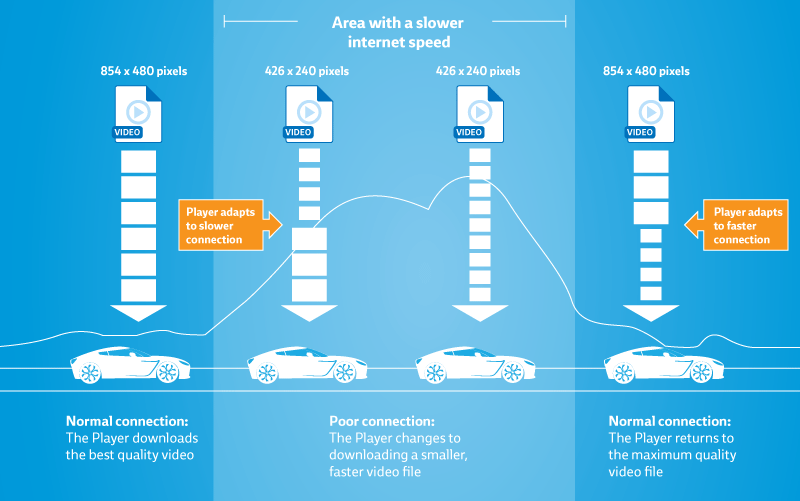
\includegraphics[scale=0.29]{figures/abs.png}\\
	\caption{Adaptive Bitrate Streaming switching video resolution \cite{abs}}
	\label{fig:abs}
\end{figure}

When a video file is encoded into an adaptive format, it is broken up into segments.
These are short snippets of video, often set to 4 seconds long (although they can be longer or shorter). At the end of each 4-second segment, the Player can switch to a different video file if necessary.

\subsection{HTTP Live Streaming}
HTTP Live Streaming (HLS) is an adaptive streaming communications protocol created by Apple. It uses the m3u8 manifest format. It provides a reliable, cost-effective means of delivering continuous and long-form video over the Internet. HLS allows a receiver to adapt the bit rate of the media to the current network conditions to maintain uninterrupted playback at the best possible quality.
  
HLS video streams are broken up into segments of data (also called chunks or packets) rather than being delivered as a continuous flow of information. To deliver the highest-quality stream possible to everyone watching, including those with small screens and poor connections, HLS streaming dynamically adapts the resolution to each individual’s circumstances. \cite{wowza}
   
In a typical HLS workflow, a video encoder solution that supports HLS receives a live video feed or distribution-ready media file. The encoder creates multiple versions (known as variants) of the audio/video at different bit rates, resolutions, and quality levels. The encoder then segments the variants into a series of small files, called media segments. At the same time, the encoder creates a media playlist file for each variant containing a list of URLs pointing to the variant’s media segments. The encoder also creates a master playlist file, containing a list of the URLs to variant media playlists, and descriptive tags to control the playback behavior of the stream. \cite{applehls} 

\subsection{Definitions}

We are going to mention some definitions \cite{refs} that will be used frequently in the upcoming sections to describe our approach. 

\subsubsection{.M3U8 Manifest File}

HLS video segments are indexed into a media playlist so that the video player understands how to organize the data. A master .m3u8 playlist file must also be created to instruct the player on how to jump between the variant-specific playlists. This is also referred to as the manifest file. \cite{wowza}

\subsubsection{Playlist}
A Playlist is either a Media Playlist or a Master Playlist.  Both are UTF-8 text files containing URIs and descriptive tags. Each Playlist file must be identified either by the path component of its URI or by HTTP Content-Type.  In the first case, the path must end with either .m3u8 or .m3u.  In the second, the HTTP Content-Type must be "application/vnd.apple.mpegurl" or "audio/mpegurl".
   
\subsubsection{Master Playlist}

A Master Playlist provides a set of Variant Streams, each of which describes a different version of the same content. A Playlist is a Master Playlist if all URI lines in the Playlist identify Media Playlists.
   
The master playlist provides an address for each media playlist in the stream. Figure \ref{fig:masterpl} shows this relationship. The master playlist also provides important details such as bandwidth, resolution, and codecs. The player uses that information to decide the most appropriate variant for the device and the currently measured, available bandwidth. \cite{applehls}

\begin{figure}[!ht]
	\centering
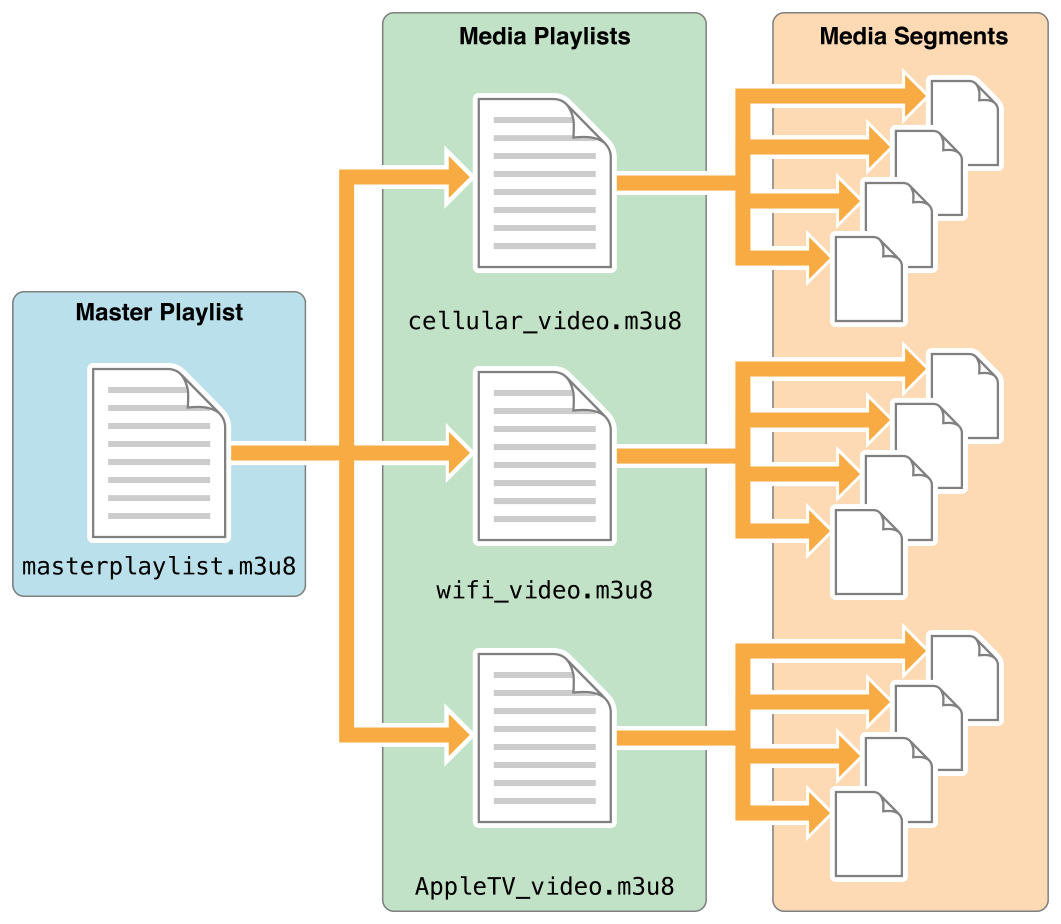
\includegraphics[scale=0.23]{figures/masterplaylist.png}\\
	\caption{Playlist relationships \cite{applehls}}
	\label{fig:masterpl}
\end{figure}
   
The following sample master playlist shows four variants. The player begins downloading the first variant it can play. If conditions warrant, the player switches to another media playlist midstream.

\begin{verbatim}
#EXTM3U
#EXT-X-VERSION:6
#EXT-X-STREAM-INF:BANDWIDTH=2855600,
RESOLUTION=960x540
live/medium.m3u8
#EXT-X-STREAM-INF:BANDWIDTH=5605600,
RESOLUTION=1280x720
live/high.m3u8
#EXT-X-STREAM-INF:BANDWIDTH=1755600,
RESOLUTION=640x360
live/low.m3u8
#EXT-X-STREAM-INF:BANDWIDTH=545600,
RESOLUTION=416x234
live/cellular.m3u8
\end{verbatim}

\subsubsection{Media Playlist}

A Media Playlist contains a list of Media Segments, which, when played sequentially, will play the multimedia presentation. The media playlists contain URLs to the media segments and other information needed for playback. 
   
Here is an example of a Media Playlist:
\begin{verbatim}
#EXTM3U
#EXT-X-TARGETDURATION:10
#EXTINF:9.009,
http://media.example.com/first.ts
#EXTINF:9.009,
http://media.example.com/second.ts
#EXTINF:3.003,
http://media.example.com/third.ts
\end{verbatim}
   
The first line is the format identifier tag \#EXTM3U. The line containing \#EXT-X-TARGETDURATION says that all Media Segments will be 10 seconds long or less.  Then, three Media Segments are declared. The first and second are 9.009 seconds long; the third is 3.003 seconds.

To play this Playlist, the client first downloads it and then downloads and plays each Media Segment declared within it. A Playlist is a Media Playlist if all URI lines in the Playlist identify Media Segments. The encoder creates the media playlists as text files saved in the M3U format (.m3u8). \cite{applehls}

\subsubsection{Variant Stream}

A Variant Stream includes a Media Playlist that specifies media encoded at a particular bit rate, in a particular format, and at a particular resolution. Clients should switch between different Variant Streams to adapt to network conditions.

\subsubsection{Renditions}

A Variant Stream can also specify a set of Renditions. Renditions are alternate versions of the content, such as audio produced in different languages.

\subsubsection{Media Segment}

A Media Playlist contains a series of Media Segments that make up the overall presentation.  A Media Segment is specified by a URI. The duration of each Media Segment is indicated in the Media Playlist by its EXTINF tag. An encoder creates media segments by dividing the event data into short MPEG-2 transport stream files (.ts). Typically, the files contain H.264 video or AAC audio with a duration of 5 to 10 seconds each. 